ss[11pt]{article}

\usepackage[margin=0.75in]{geometry}
\usepackage{graphicx}
\graphicspath{ {images/} }

\title{fMRI Dataset from Complex Natural Simulation with \emph{Forrest Gump}: \\A Restudy}
\author{
  Chang, Jordeen\\
  \texttt{jodreen}
  \and
  Daks, Alon\\
  \texttt{AlonDaks}
  \and
  Luo, Ying\\
  \texttt{yingtluo}
  \and
  Yu, Lisa Ann\\
  \texttt{lisaannyu}
}

\bibliographystyle{siam}

\begin{document}
\maketitle

\abstract{Most fMRI studies use highly simplified stimuli that are very
different from what people experience in everyday life. "A High-Resolution 7-
Tesla fMRI Dataset from Complex Natural Stimulation with an Audio Movie" by
Hanke et al. sought to create a dataset of naturally occurring brain states
by exposing participants to a more complex stimulus, the audio description of
\emph{Forrest Gump}. This particular audio description allows for the study of
auditory attention and cognition, language and music perception, and retrieval
of explicit memory without the effect of visual imagery. Furthermore, the
study was conducted on 20 subjects enabling research into brain similarities
among individuals when exposed to the same complex stimulus. The goal of our
paper is to first reproduce a subset of the analysis conducted by Hanke et
al., then apply machine learning to see if we can predict if a subject was
listening to a day or night scene of the movie based on brain state.}

\section{Introduction}

The main purpose of the original study was to examine properties of brain
response patterns that are supposedly common when people are exposed to audio
and movie simulation. We intend to replicate their experiment using the data
they gathered from the 20 participants. For example, a BOLD time-series
similarity measure (e.g. correlation) is often used to quantify similarities
in responses among individuals. Hanke et al. recognized that this was a common
approach, but they went beyond that and also implemented representational
similarity analysis  (RSA). To replicate their analysis, we will create 
dissimilarity matrices for 18 individuals using the same searchlight mapping 
approach that they used (Subjects 4 and 10 were not included due to missing 
data). Doing so will capture 2nd-order isomorphisms in response patterns. 
Lastly, to access statistical significance, we will transform the 
representational consistency map into percent rank with respect to the total 
distribution of the DSM correlations. We'll calculate the mean correlation 
coefficient and compare our value to theirs.

Before we formally began, we performed basic sanity checks on the data. We
downloaded and loaded the files successfully, and we have confirmed that we
have data for every test subject. Because there were various versions of the
data (e.g. linear vs. non-linear), we had to first isolate which dataset best
suited our needs. The non-linear alignment had more smoothing than the linear
alignment, which made that dataset more appropriate for initial exploratory
data analysis.  We recognize that the non-linear alignment is crude, since it
probably was conducted with no specific hypothesis about which parts of the
brain should be expanded or compressed, but not having the machinery or
background to better preprocess the data, we at first simply used the non-linear
alignment version of the data provided by Hanke et al.
\cite{hank2014audiomovie}.

Reproducibility is crucial in research, especially when such high volumes of
data are involved, because it allows other people to fact-check the work. When
people collaborate, new insights can be shed and the rate of progress is
expedited. For this study, we began by extracting data we see fitting and
asking questions that were not addressed by the original study. To answer
these questions, we utilized neuroscience concepts, additional packages, and
parallel processing techniques. We found that in certain functions, such as
parsing through csv files, it would have been easier to hard code in the
correct values. However, hard coding would have defeated the reproducibility
aspect of our study because our code would break if the data were slightly
modified.

A central theme of the course is exploring reproducible practices while conducting scientific research. For our project we address reproducibility 
from two perspectives: first, we designed our code and scripts to be modular 
and portable so that anyone with an appropriate computer can rerun our analysis 
and reproduce the results we cite in this paper. Second, we attempted to reproduce 
some of the results cited in the original paper by emulating Hanke et al.\'s 
technique and comparing values. 

\section{Data}

The data is curated and segmented into 20 .TGZ files, where each of the 20
.TGZ  files corresponds to one of the 20 subjects in the experiment. Each
subject  accounts for approximately 16 GBs of data. We verified the usability
of the data by inspecting and loading data corresponding to subject 1. We
limited our initial exploration to a single subject since downloading each
.TGZ takes  approximately one hour.  The download for each subject includes a
lot of other information besides just the fMRI data, such as cardiac and
respiratory trace, angiographies, and structural MRI data. Each subject's fMRI
data includes several formats: Raw BOLD functional MRI, Raw BOLD functional
MRI (with applied distortion correction), Raw BOLD functional MRI (linear
anatomical alignment), and Raw BOLD functional MRI (non-linear anatomical
alignment). The corrected and aligned versions of the data attempt to
eliminate device and scan related noise. Scan data is accessible in nibabel
compatible formats (.NII).

In addition to data for each subject, there was also data about the
experiment as a whole, including a German audio description of the stimulus
and a csv file with scene information, including the timestamp of the
beginning of each scene, the scene location, whether the scene took place
during the day or night, and whether the scene was interior or exterior.  

\subsection{Extracting Data} 
\begin{center}                                                                  
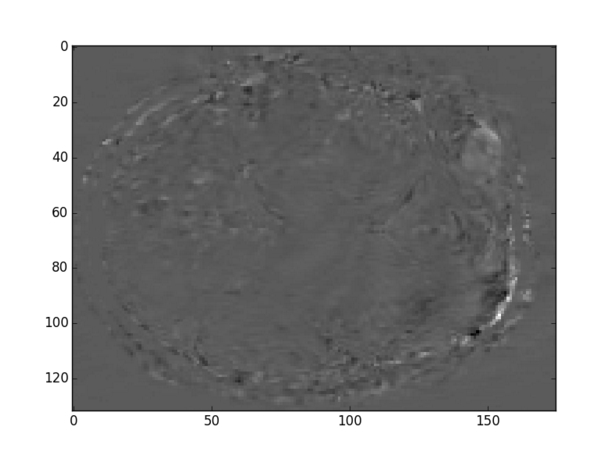
\includegraphics[height=8cm]{1}                                                 
\end{center}                                                                    
                                                                                
With regard to our day/night prediction analysis, we will be only working with  
the first subject for now for testing purposes, but if time had allowed, we     
would have ran our code on a couple of other subjects for comparison testing.   
However, for our reproduction analysis, we will be working with five subjects.  
To ensure speedy access to other subjects' datasets, our strategy for getting all 
the data entails each group member spending downloading a different quarter of the 
overall dataset, and then locally transferring the remaining three-quarters of the 
data from our hard drives.  After downloading the data for all twenty subjects, we 
found the data online at studyforrest.org, which allowed us to only download the 
files we needed, as opposed to the entire datafile for each subject.  

We will not be using all of the data. The data files are very large: for each 
subject, the download size is approximately 16 GB, and that does not even 
include unzipping all the file inside. Given that we have twenty subjects, 
downloading all of this could be a paper in it of itself. Since the focus of 
this class is mainly fMRI data, we decided to ignore everything else. However, 
the fMRI data is still not of a trivial size because three versions of the data 
are included: the raw data, the linear alignment, and the non-linear alignment.   

At first, we used the non-linearly aligned data provided by Hanke et al, as
mentioned above.  However, after talking to Matthew Brett, about these plots, 
we decided to use the data kindly preprocessed by Russ Poldrack and the OpenfMRI 
group.  
\begin{center}                                                                  
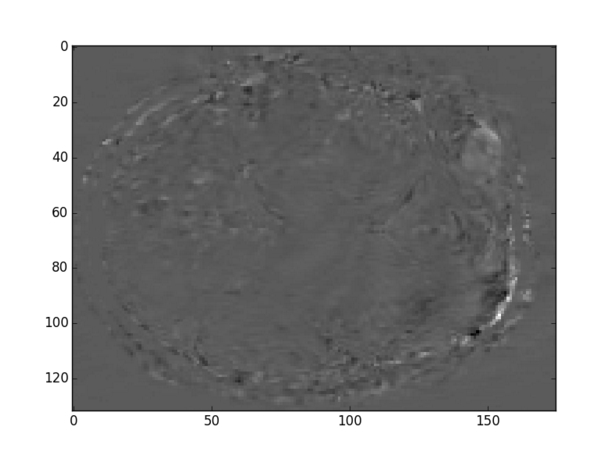
\includegraphics[height=8cm]{1}                                                 
\end{center}    

\begin{center}                                                                  
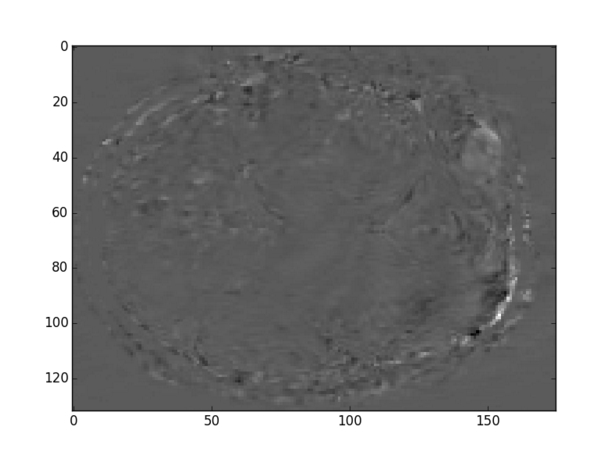
\includegraphics[height=8cm]{1}                                                 
\end{center}    
There appears to be an artifact in the data.  This image is supposed to show 
the day/night regressor. It is remarkably gray both inside and outside the 
head.  This is certainly possibly, since not every voxel will have a signal
difference between day and night volumes.  However, this image also looks 
nearly identical to the linear drift image, which seems to indicate great
activation in the scalp.  After reading how Hanke et al. corrected for motion,
namely, adjusting the scanner itself when participants moved, instead of 
modeling for their motion, which is less prone to error, Matthew suggested we
use the OpenfMRI data, which corrects for motion using a highpass filter.

The original scenes file contained an error: one scene was labeled 'DAY' for 
the interior/exterior column.  We contacted Hanke, and he told us the correct 
label: 'EXT' for that scene.     
   
\subsection{Preprocessing Data}                      

Hanke et al. preprocessed the data for us by creating an EPI group template.    
They aligned each image to the first image for each individual, then aligned    
all brains using FLIRT.  However, we thought it would still be a good idea to   
model the noise created by linear drift.  This subject moved backwards and to   
the left, but the data does look quite messy.  It appears as though the fMRI    
is picking up signal from outside the subject\'s head.

\subsubsection{Concatenating Across Runs}
Due to the length of the movie, the stimulus was split up into eight segments,  
each approximately fifteen minutes long, and each participant listened to four  
segments on two separate days while lying in the fMRI scanner.  At every        
segment boundary except for the first, Hanke et al. repeated at least the last 
six seconds between the beginning and end of each segment so there would be a 
short overlap between segments.  They also removed the first and last four 
volumes of the data for each run, presumably to account for the overlap 
between segments, although it is not entirely clear from their article.  In 
order to have more data for our machine learning training set, and in order to 
more easily determine which volumes took place during the day and which took 
place during the night, we concatenated the eight runs together and removed the
first and last four volumes of each run, as Hanke et al. did with their data.

\subsubsection{Smoothing}

We smoothed the data before performing any analyses by applying a Gaussian      
filter.  While filters may smooth temporally or spatially, we have chosen to    
only smooth spatially, as the temporal signal is already noisy.  This spatial  
filter smooths the signal between adjacent voxels, addressing                   
our assumption that adjacent voxels are not independent.  The   
Gaussian filter from the scipy.ndimage module smooths the data in terms of      
standard deviation.  It is conventional in fMRI studies to smooth in terms of mm, 
so we first had to convert mm into SDs in order to apply this  
Gaussian filter.

There are two versions of smooth data, one for the reproduction analysis, and
one for the classification analysis.  We smoothed using 8 mm along each axis
for the reproduction analysis, and 4 mm along each axis for the classification
analysis.  For the reproduction analysis, we are taking correlations between
voxels, so we want to make sure we have the right signal for each voxel.  For the classification analysis, we just want to be able to remove the noise, so we 
applied a much more conservative filter.

\subsubsection{Reshaping}
Once we have preprocessed the data by concatenating the data and smoothing it,
we reshape it to a 2D array: number of voxels (1,110,800) by time (3543).

\section{Methods}

\subsection{Reproduction}

The original paper focused on inter-individual response pattern similarity. In
other words, their analysis measures brain pattern correlation between
subjects who listened to \emph{Forrest Gump}. Hanke et al. identifies two 
methods for measuring correlation. The first method takes the BOLD time-series 
and calculates the voxel-wise Pearson correlation and the second method employs
\'representational similarity analysis to identify 2nd-order isomorphisms in
the response patterns across brains.\' Since the first technique is simpler, we
chose that to be the portion of the analysis we tried to reproduce. Although
20 subjects were scanned, Hanke et al. excluded subjects 4 and 10 from the 
paper since data was missing. With the 18 remaining subjects there are 153 
pairs (18 choose 2) for which voxel-wise correlations are calculated. Hanke et 
al. calculated correlations on linearly and non-linearly aligned raw data. 
Instead of using the paper\'s raw data, which was applied through a bandpass 
filter, we used a version of the raw data provided by the OpenfMRI group which 
was non-linearly aligned and applied through a highpass filter.

The main challenge in reproducing the paper\'s analysis resides in the large
amount of data that must be processed. Since subjects were scanned at 7 Tesla,
the brain images have a very high resolution, and therefore are large. The
full two hour scan for each subject is approximately 7.5 GBs, meaning 153
pairs of 2 x 7.5 GB files must be processed. A seemingly trivial calculation
of computing correlations between a set of voxels is difficult at this paper\'s
scale. On an Intel core i7 (1.7 GHz) machine with 8 GBs of RAM, preprocessing
(concatenating runs and converting the 4D image to 2D) takes approximately 30
minutes per subject. Calculating the correlations between a pair of subjects
takes 10 minutes (8 minutes to load both subjects time courses into memory and
2 minutes to calculate the Pearson correlations for all the voxels).  To
combat these concerns, we used python\'s multiprocessing module to parallelize
the reshaping of 4D to 2D arrays in the preprocessing step and parallelize the
calculating of correlations between subjects. Additionally, we ran our
analysis on Amazon EC2 instances with memory capacities large enough to fully
load both two hour time courses for each subject in the pair being considered.
By renting multiple EC2 instances, we are able to parallelize the
preprocessing work enabling multiple subjects to be preprocessed once.

Since rerunning our preprocessing and correlation code may take several hours
depending on one\'s machine, we defined a UNIX environment variable called
STAT159\_CACHED\_DATA. If this variable is set to \'True\', then our python
scripts will look to see if preprocessed versions of the data exist in the
/data/processed directory and use those instead of recomputing them. If
however one wants to fully recompute everything, merely setting
STAT159\_CACHED\_DATA to \'False\' will ensure that all python scripts do not
use data files that have already been computing. If the user does not specify
STAT159\_CACHED\_DATA, the default behavior is to use cached files. Enabling
the user to easily choose whether or not to recompute intermediary data files
is consistent with the reproducible paradigm this course emphasizes.

Because of our memory and storage limitations, we decided to only calculate 
correlations between five subjects.  Thus, we will have 10 pairs (5 choose 2) 
in total, between each combination of those five subjects, rather than the 153
(18 choose 2) pairs Hanke et al. used.  We did not believe we would lose much
information by running the analysis on just five subjects rather than eighteen.
Thus, our voxel-wise inter-brain correlation was determined for 10 pairs as the 
Pearson correlation of the time courses for all voxels, a total of 1,108,800.
Hanke et al. reported values for the pooled and means voxel-wise inter-individual 
correlation at various percentiles for both the linear and non-linear 
anatomical alignments.  

We will be running the inter-brain correlations for these 10 pairs at the 
levels using the preprocessed data provided by Poldrack and the OpenfMRI project, 
and will compare our result at the 0, 25, 50, 75, 90, 95, 99, 99.5, and 100\%
percentiles to that of Hanke et al.

Simply concatenating the eight runs together led to a runs effect, since there
is some variability due to the signal coming from the same run. To correct for 
this, we took our 2D data of voxels against time (V x T), and took the difference 
between signal from one volume to another, giving us a 2D array of V x (T-1), or
1,110,880 by 3542. To get a measure of the signal of the brain at every point in
time, we took the RMS across all voxels for a particular time to get a 1D array 
of length (T-1), or 3542. 

\begin{center}                                                                  
\includegraphics[height=8cm]{9}                                                 
\end{center}   

To demonstrate this effect, we plotted the RMS error for each of 3542 points.  
This plot shows the runs effect from subject 1.  There are seven clear spikes, 
representing the seven points between runs.  The highest point is the fourth 
one, which is the point between the first day of fMRI imaging and the second
day.  Thus, it is clear that there is a difference in signal between runs and
we need to correct for it.  

We correct for the runs effect by taking the average of the correlation 
coefficients across each run.  To demonstrate how we came to this solution, 
we ran a simulation with just two runs of 100 time points each for just two 
subjects, using a signal mean of 5 for the first run and 10 for the second.  
\begin{center}                                                                  
\includegraphics[height=8cm]{10} 
\end{center}  
The correlation between the 2 subjects across the entire run is 0.6336, which
seems relatively high, indicating that the subjects' voxels are activated 
roughly the same amount at the same times.  However, there is a confounding
factor of the difference in signal between the two runs.  To investigate that
confounding factor, we looked at the correlations within each run separately.  
The correlation between the two subjects within the first run is -0.236, and 
the correlation between the two subjects within the second run is 0.0883.  
Thus, the relatively high overall correlation of 0.6336 between the 2 subjects 
is actually a measure of the difference between runs, not the correlation 
between subjects.  To solve this problem, we will take the average across the 8
runs to be the correlation coefficient.

We calculate the correlation coefficient for each pair and plot the entire
distribution.  There are two versions of the correlation coefficient 
distribution.  The first is pooled, which dumps all correlations together, 
and the second is mean, which takes the average of all voxel correlations.  
Thus, there are 10 times the voxel correlations for the pooled version as for 
the mean version.

From those two distributions, we calculate the correlation coefficient at
various percentiles, including 0, 25, 50, 75, 90, 95, 99, 99.5, and 100\%,
for both the pooled and mean correlation coefficient distributions.

\subsection{Results}

\begin{center}                                                                  
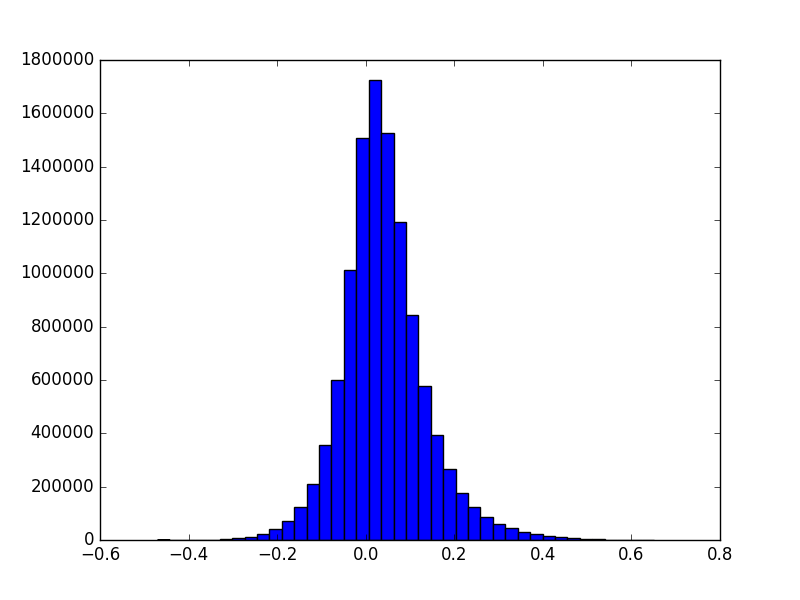
\includegraphics[height=8cm]{pooled_correlation_histogram} 
\end{center}  
Pooled correlation
\begin{center}                                                                  
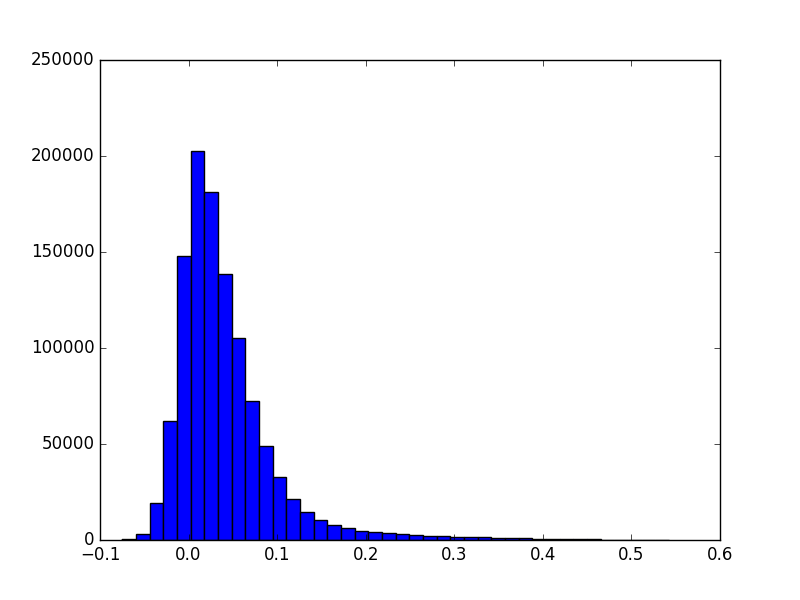
\includegraphics[height=8cm]{mean_correlation_histogram} 
\end{center}  
Mean correlation

These correlation coefficients are both centered slightly right of
0, which we expect, since we expect there to be a weak inter-subject
correlation for most voxels.

From those correlation coefficient distributions, we calculated the 
correlation coefficients at the 0, 25, 50, 75, 90, 95, 99, 99.5, and 100\%
percentiles, as can be seen in the table below.
\begin{table}[h!]
  \centering
  \caption{Our Results}
  \label{tab:table1}
  \begin{tabular}{cccccccccc}
    percentile & 0 & 25 & 50 & 75 & 90 & 95 & 99 & 99.5 & 100\\
    \hline
    pooled & -0.470 & -0.015 & 0.032 & 0.088 & 0.156 & 0.208 & 0.333 & 0.384 & 0.652\\
    \hline
    mean & -0.075 & 0.006 & 0.027 & 0.059 & 0.101 & 0.143 & 0.291 & 0.347 & 0.543\\
  \end{tabular}
\end{table}

\begin{table}[h!]
  \centering
  \caption{Results reported by Hanke et al.}
  \label{tab:table1}
  \begin{tabular}{cccccccccc}
    percentile & 0 & 25 & 50 & 75 & 90 & 95 & 99 & 99.5 & 100\\
    \hline
    pooled & −0.412 & −0.013 & 0.008 & 0.031 & 0.056 & 0.078 & 0.163 & 0.207 & 0.719\\
    \hline
    mean & −0.008 & 0.002 & 0.005 & 0.013 & 0.032 & 0.052 & 0.103 & 0.126 & 0.269\\
  \end{tabular}
\end{table}

Our correlations appear to differ from Hanke et al.'s reported numbers.  In 
general, our numbers are higher than theirs, and for the 0 and 25th percentiles, 
we report negative pooled correlations, while all of theirs are positive.

Once we had that correlation coefficient information, we applied a threshold of 
percentile rank of 95\% to get voxels with a relatively high correlation 
coefficient.  In our data, the 95th percentile corresponds to r = 0.0143 for 
the mean correlation coefficient distribution.  Voxels with a correlation
coefficient above this threshold were coded blue, and all other points 
were coded gray, as shown below.  The areas of the brain that are blue
are similar to the areas shown in Hanke et al.'s paper, namely, the
Planum Temporale (PT) in both hemispheres.  According to Hanke et al., 
that region is known to be involved in "processing complex sounds and
speech," such as one might hear while listening to an auditory movie.

\subsubsection{Discussion}

We have a few hypotheses as to why our correlation coefficients are 
higher than those reported by Hanke et al.  1) We used 
different motion-corrected data: they used a bandpass filter, while we 
used the preprocessed data provided by Matthew, which used a highpass
filter.  2) We used a Gaussian filter to smooth the data; they do not 
indicate using any filter to smooth the data in their paper.  Smoothing 
spatially should increase the correlation between subjects, possibly 
explaining why our correlations are all higher than theirs.  3) We 
took the average of the correlation for each run to account for the runs
effect; they did not.  However, we expect that taking the average of 
the correlation for each run would lower the overall correlation, so
this hypothesis is not supported by our data, where our correlations
are higher than all of theirs.   4) Their correlations may be incorrect.
The values they reported for mean correlation coefficients in their 
written text of the paper do not line up with the values they report in 
their table.  For example, Hanke et al. reports the mean correlation 
coefficient values at the 95\% level as r = 0.076 (linear) and r = 0.078 
(non-linear) at the supplemental table shown online at
http://www.nature.com/articles/sdata20143/tables/5, and r = .077 (linear) 
and r = .086 (non-linear) in the paper.  We contacted Hanke, and he acknowledged 
the discrepancy, but has yet to get back to us on which is the correct value.  

\subsection{Classification of Day/Night}

In addition to reproducing Hanke et al.'s analysis, we also wanted to
conduct our own, based on personal interest and ability.

After perusing all the stimulus related data (e.g. data annotating each 
\emph{Forest Gump} scene and when a subject was exposed to
that scene), we decided to guide part of our analysis to see if we could
summarize any interesting trends in fMRI response with respect to these
features. Additionally, by investigating a single subject for our initial
analysis  and using the non-linearly aligned transformed data, we have limited
our project\'s scope to approximately 5 gigabytes from the roughly 320
gigabytes that were published with the paper. With the data reduced to a
manageable state, we have successfully overcome this obstacle. Finally, by
introducing a data\_path.json file to reference where each raw data file is
located, we have designed a clean schema for our python scripts to find and
load data in the project repository.

Our initial plan was to first just conduct some basic exploratory data
analysis and then further delve into the findings that strike us as intriguing
or unusual. We began by writing functions that loaded the .nii files for each
subject and calculated and plotted the standard deviations across voxels.
After exploring the files provided by Hanke et al., we saw that there exists a
csv file of the scenes in the movie with a time-stamp, a brief scene
description, whether it takes place in day or night, and if it is inside or
outside, as mentioned in the Data section.

We used this information and the fMRI data to select features with the goal of
building the best possible predictor of certain aspects of a movie scene given
fMRI data. We wanted to be able to accurately predict whether a particular
movie scene falls under one of two categories: day or night.  Our plan of 
action was to 1) select voxels that seemed to differ most between the two 
groups as features, and 2) use machine learning to classify volumes as 
beloning to one of two groups (i.e. day or night).

We began with the analysis for differentiating day and night slices, but this
analysis can easily be applied to address the question of which voxels pick up
on the difference between interior and exterior slices.  We can then use
machine learning to predict which slices are interior and which are exterior.

After determining which points in time were during the day and which were
during the night, and which were inside and which were outside, we can perform
a t-test to determine if the signal is significantly different between each of
the two groups for each voxel.  We will perform a multiple comparisons test to
correct for the number of t-tests we will be running.   We will also model
each of those voxels that are statistically significant to see what their time
courses look like.

To select voxels as features for our classification problem, we first
determined which slices took place during the day and which took place during
the night, which were inside and which were outside.  In order to account for
baseline BOLD and any linear drift created by the subject moving in the
scanner, we created a design matrix.  The design matrix currently includes 4
columns: a column for day vs. night, a column for linear drift, and a column 
of ones for the intercept.

\begin{center}
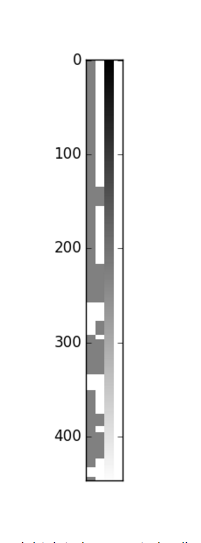
\includegraphics[height=8cm]{2}
\end{center}

The figure above shows the design matrix, including day vs. night, linear drift, and a column of ones for the intercept

We then performed a t-test for each voxel to determine if the signal is
significantly different between each of the two groups we were comparing.
This gave us an array of t-statistics, one for each voxel, a total of 1108800,
as well as an array of betas, telling us the effect size.  Since we wanted to
pick out the voxels with the biggest change between groups, we cut down that
number by selecting the top portion of them.  This number of feature
selections is rather arbitrary, but should be relatively small so we can
create a random forest with it that does not overfit.  Part of our analysis is
determining the optimal number of features to select. This will be done via
cross validation.

\begin{center}
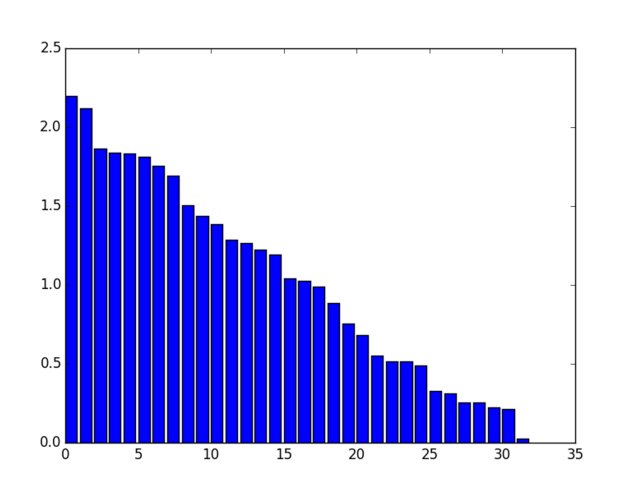
\includegraphics[height=8cm]{3}
\end{center}

The figure above is the largest 32 t-statistics.

The time course for the voxel with the highest t-statistic looks very noisy.
We can compare it to the stimulus (day) time course, but there is no obvious
relationship.


\begin{center}
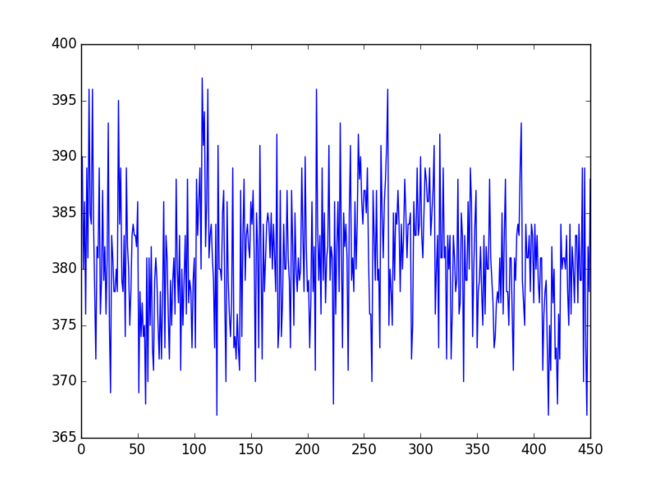
\includegraphics[height=8cm]{4}
\end{center}

The figure is the time course for the voxel with the highest t-statistic.

\begin{center}
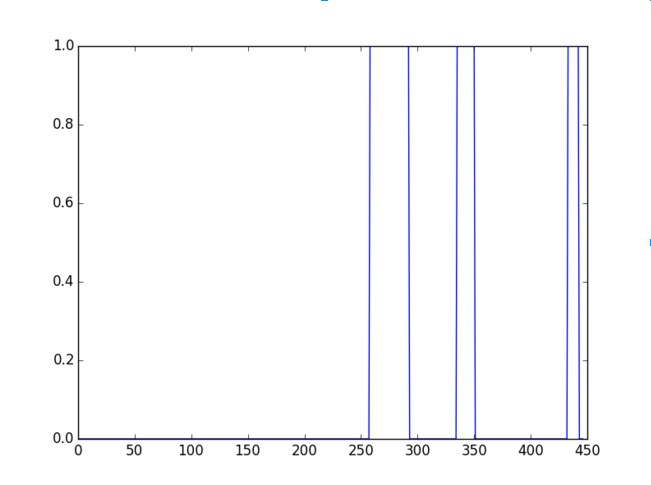
\includegraphics[height=8cm]{5}
\end{center}

The fiture is the day-night time course for Task 1, Run 1.  Very few scenes
take place at night for this run.

Because we are ultimately interested in feature selection, not in whether
certain voxels are significantly different between the two groups, we did not
correct for multiple comparisons.  If we were interested in the significance
of certain voxels, we would apply a Bonferroni correction.

We wanted to know which areas of the brain seemed to be most inclined to pick
up on the difference between day and night.  Thus, we plotted the betas
testing the hypothesis that there is no difference between day and night for
each voxel.  Unfortunately, this looks very similar to our linear drift image,
where there appears to be an artifact.

\begin{center}
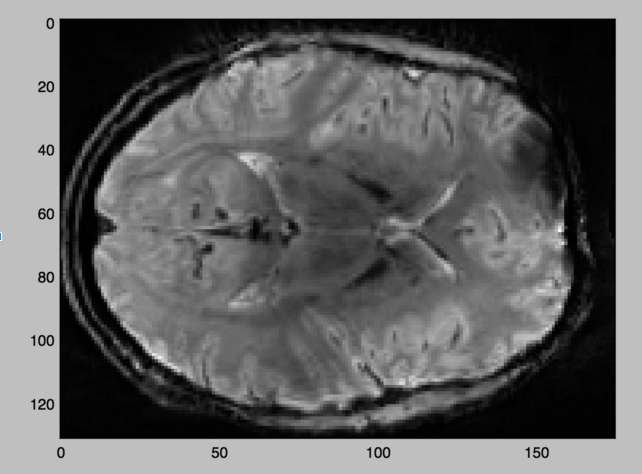
\includegraphics[height=8cm]{7}
\end{center}

We can also apply this to the question of whether we can tell the difference
between positive, negative, and neutral scenes by examining certain voxels in
the brain. Unlike the scenes data, which we can only code as day, night,
interior, or exterior, since that is all the information we have, since we are
extrapolating the sentiment of the scene from the scenes descriptions
ourselves and sentiments can vary along a spectrum from very positive to very
negative, we can perform a linear regression with sentiments.  We only coded
the sentiment for scenes in which a narrator was speaking, and only the time
in which he was speaking.

To see if we could predict whether a slice was taken from a day or night
scene, we focused on creating a random forest, using voxels selected as the
features as the nodes.  We first trained on a random 80\% of the slices,
collapsing day slices and night slices together, so that the distribution of
the slices selected was roughly equivalent to the distribution of the entire
data, rather than selecting 80\% of the day slices and 80\% of the night
slices.  The other 20\% of the slices we preserved to be our testing set.  We
created a decision tree, which we used to predict whether each slice in the
testing set took place during the day or the night.  In theory, we could use
the first six runs as the training set, and see how well they predict the last
two runs for a given participant.


\subsection{Analysis} 




\section{Results}

We began our exploratory data analysis by writing functions
that plot a slice of the brain at any given time and the standard deviations
across voxels for individual subjects using Matplotlib. This enabled us, at a
quick glance, to gauge the variability of the fMRI data.

\begin{center}
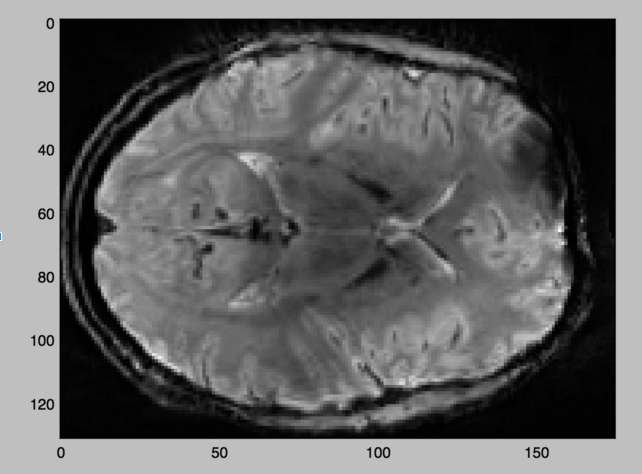
\includegraphics[height=8cm]{7}
\end{center}

It takes a few minutes to calculate the standard deviation for each volume in
the 4D array for Subject 1's Task 1, Run 1. This makes sense, as the 4D
array is (132, 175, 48, 451) in dimension; this means we are calculating and
plotting 451 standard deviations in total. From the plot above, we can see
that for this particular run and task, the standard deviations across all 451
points is within 171 and 173.5. Though this range may seem small, from the
plot we can see that there is quite of variability within that range of 2.5.
One possible explanation for this is the varying responses to different movie
scenes. Some scenes will evoke different reactions and thus different values
per voxels.

\begin{center}
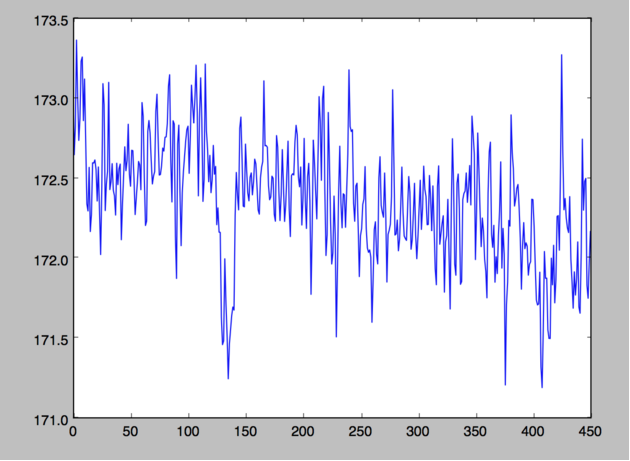
\includegraphics[height=8cm]{8}
\end{center}

One initial direction we had hoped to explore was possible differences in
physiological responses to certain movie scenes by gender and age. However, we
later had to forgo this idea because doing so required us to process and
analyze the entire dataset, something that we could not efficiently do given
our limited computing resources. To be more specific, we would have had to
comb through around 16 gigabytes worth of data just for one subject. Though
these were certainly interesting questions, their focus was too broad for us
to be able to fully address them.

So, in order to glean anything remotely useful, we had to narrow down our
focus. There are 20 subjects with 8 runs each. We limited our initial analysis
to just one run for one subject in order to conduct hypothesis tests. And
after parsing the two csv files (scenes.csv and demographics.csv), we then had
limited data about the movie scenes and personnel about each subject. We
implemented "Scene Slicer" and "Subject" classes with attributes that were
unique to each scene or subject.

Out of the 451 recorded instances of whether a scene was day or night for
Subject 1 and Task 1, \emph{Forrest Gump} had 390 day slices and 61 night slices and 296 interior slices and 155 exterior slices. Subject 1 is a male 
who is 30-35 years old and had seen the movie 5 times prior to the study.

Though there were much more data in the demographics.csv file than the
attributes given to a Subject object, we had deemed those data to be
irrelevant for our purposes. For example, there were also data about each
subject\'s music preferences and languages spoken. As we suggested before,
there were a lot of directions that we could have taken with all this data,
but these directions were too general and broad for us to be able to use them
in conjunction with the fMRI data to do any conclusive studies.

The decision tree we created had a prediction accuracy of 83.5\%.  However,
86.5\% of slices took place during the day, so this first tree is performing
worse than chance.

\section{Discussion}

\subsection{Interpretations and Implications}
what does this mean? both this study and in general
\subsection{Potential Future Studies}

Since the 20 participants have differing amounts of exposure to \emph{Forrest 
Gump}, with some participants having never seen the movie before and one 
participant who had seen the movie twelve times before, a future study could 
examine the difference in voxel activation between participants who had never 
seen the movie before and those with high amounts of exposure.

Ideally, a future investigator could split the participants into a training
set and testing set, and predict which participants have limited familiarity
with the movie, defined as seeing the movie 2 or fewer times.  However, there
are a relatively small number of participants, only 20, since fMRI is
expensive, so the predictive ability of that study would be rather limited.


\bibliography{project}

\end{document}

